% Badger
\documentclass{article}
\usepackage{tikz}

\begin{document}

\begin{center}
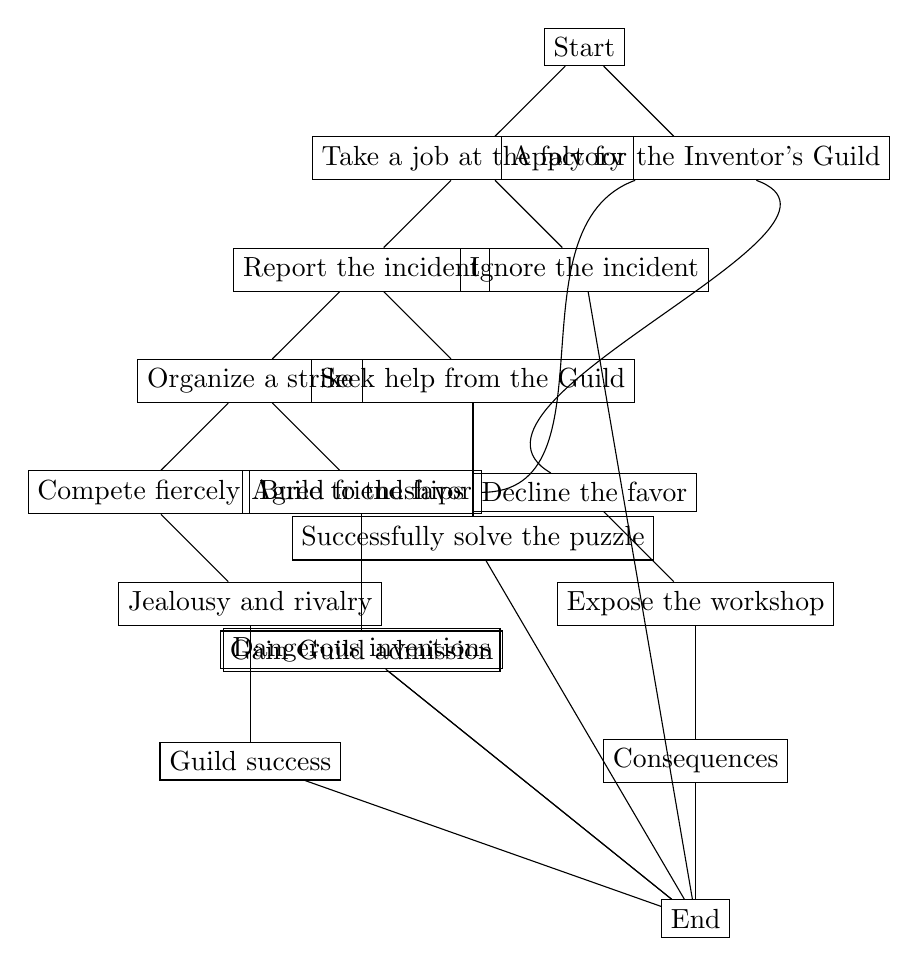
\begin{tikzpicture}[
    node distance = 2cm,
    every node/.style={draw, rectangle, align=center},
    edge from parent/.style={->, >=stealth, shorten >=1pt, semithick, black}
]

% Nodes
\node (start) {Start};
\node [below left of=start] (factory) {Take a job at the factory};
\node [below right of=start] (guild) {Apply for the Inventor's Guild};
\node [below left of=factory] (report) {Report the incident};
\node [below right of=factory] (ignore) {Ignore the incident};
\node [below left of=report] (strike) {Organize a strike};
\node [below right of=report] (help) {Seek help from the Guild};
\node [below of=help] (success) {Successfully solve the puzzle};
\node [below left of=strike] (compete) {Compete fiercely};
\node [below right of=strike] (alliance) {Build friendships};
\node [below of=alliance] (admission) {Gain Guild admission};
\node [below right of=compete] (jealousy) {Jealousy and rivalry};
\node [below of=jealousy] (guildend) {Guild success};
\node [below left of=help] (favor) {Agree to the favor};
\node [below right of=help] (nofavor) {Decline the favor};
\node [below of=favor] (danger) {Dangerous inventions};
\node [below right of=nofavor] (expose) {Expose the workshop};
\node [below of=expose] (consequences) {Consequences};
\node [below of=consequences] (end) {End};

% Edges
\draw (start) -- (factory);
\draw (start) -- (guild);
\draw (factory) -- (report);
\draw (factory) -- (ignore);
\draw (report) -- (strike);
\draw (report) -- (help);
\draw (help) -- (success);
\draw (strike) -- (compete);
\draw (strike) -- (alliance);
\draw (compete) -- (jealousy);
\draw (alliance) -- (admission);
\draw (jealousy) -- (guildend);
\draw (guildend) -- (end);
\draw (success) -- (end);
\draw (ignore) -- (end);
\draw (admission) -- (end);
\draw (guild) to[out=-160,in=0] (favor);
\draw (favor) -- (danger);
\draw (danger) -- (end);
\draw (guild) to[out=-20,in=150] (nofavor);
\draw (nofavor) -- (expose);
\draw (expose) -- (consequences);
\draw (consequences) -- (end);

\end{tikzpicture}
\end{center}

\end{document}